\documentclass[12pt]{article}
\usepackage[font=small,labelfont=bf]{caption}
\usepackage{graphicx}
\usepackage{url}
\usepackage[hidelinks]{hyperref}
\usepackage{subfig}
\usepackage{float}
\usepackage[margin=1in,includefoot]{geometry}
\usepackage{fancyhdr}
\usepackage[parfill]{parskip}
\pagestyle{fancy}
\renewcommand{\footrulewidth}{1pt}

\begin{document}

\begin{titlepage}
\begin{center}
\begin{figure}[t]
\hspace*{0.35cm}
\includegraphics[width=1.0\textwidth]{uclLogo}\\
\end{figure}
\line(1,0){300}\\
[0.25in]
\huge{\bfseries Scenario Week 4 }\\
\huge{\bfseries Computational Geometry Implementation }\\
[2mm]
\line(1,0){200}\\
[1.5cm]
\textsc{\LARGE University College London}\\
\textsc{\normalsize Department of Computer Science}\\
\textsc{\normalsize Group Orthrus}\\
[5cm]
\end{center}

\end{titlepage}
\tableofcontents

\newpage
\section{Introduction}\label{sec:abstract}
This report will be outlining team Orthrus's implementation for the Scenario Week 4 computational geometry problem. We will be discussing the different algorithms used, the choice of tools to build and implement the algorithms, the visualisation of the problem and the surprises we encountered during the week that we found interesting. 

\subsection{The Problem}\label{sec:theProblem}
We were introduced to an NP hard optimisation problem that naturally arises in the study of swarm robotics similar to the famous problem of "Freeze-Tag". The problem consists of robots as well as obstacles to minimise and find the most optimal path of awakening all robots in the shortest time/path possible.

\section{Language and Tools used}
\subsection{IntelliJ IDEA}
Our team decided to use Java to implement the core algorithms since it was the language that most of the team was comfortable with. We compiled the Java code using IntelliJ IDEA. The only libraries we used are the Java core libraries. 

\par
\subsection{Processing}
Since we were already using Java, it is the language that our team is most comfortable with, and the fact that we have all used Processing before, this made Processing the natural choice for visualisation. Within our visualisation the first robot is coloured red and  all the paths that robots take have been given a specific colour which can be traced to their destinations. 
\begin{figure}
	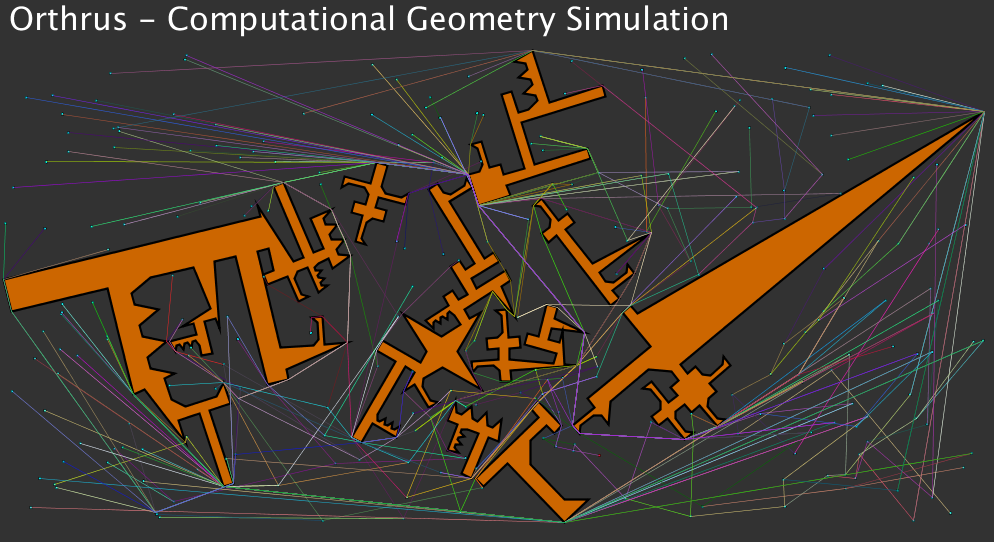
\includegraphics[width=\textwidth]{CS}
	\caption{This shows the corresponding paths between each robot within map 30 of the problem set}
	\centering
\end{figure}

\section{Geometric Algorithms}
In order to manage the complexity of the program, we used some algorithms to pre-process the inputs into a specific graph. After this was done, the problem we were solving was exactly the freeze-tag problem. 

\subsection{Stage 1: Visibility Graphs}
We implemented some code to detect collisions, that is based upon comparing straight line paths against the edges of the obstacles. This was done by checking vector intersections in a method similar to ray casting. 
\par

In order to avoid collisions, we created a list of 'visible points' for every single robot as well as all vertices of the obstacles. This was then translated into a graph, with invisible edges having a weight of 'infinity', and visible edges having their real distances. Then to find the optimal paths between each point, we used the Floyd-Warshall algorithm. 
\par

This stage allows us to create a graph that does not consider obstacles any more, and we solve the pure freeze-tag problem, as each robot has an optimal path to each other robot, and the graph created is a complete graph.

\subsection{Stage 2: Freeze Tag Problem}
Firstly, we implemented the most basic algorithm of allowing one robot to wake up every other robot, in the order that they were read into the file. This allowed us to get a valid solution very quickly, however it was far from optimal.
\par

The next optimisation we made, was to consider an A* approach; the 'best' decision is taken at each stage, in order to try to find the optimal path. This meant that one robot was still waking up every other robot (and subsequently awoken robots were still inactive), but it did it in a greedy approach which is far more optimal in most cases.
\par
 
The largest optimisation after this, was to use each robot that is awakened to take its own optimal/greedy decisions. We managed this by adding each robot 'task' to a queue based on completion time of the task (since the start, not just the time the individual job would take), and then assigning each robot the closest robot to it to wake up after it completes the task. 
\par

During the week, since our code was structured specifically for the multi-robot A* variant, we found it hard to adapt the existing code for new algorithms. However, we tried to implement a 'lookahead' of 1 when taking decisions, to try to get better choices. Another route that we tried was a method akin to agglomerative hierarchical clustering, with a variant of Kruskal's algorithm. We are confident that both work as we did trial runs on paper, however we could not successfully implement either in time.
\par

\subsection{Complexities}
\begin{itemize}
\item Each path being compared to each obstacle was O(n) in the size of the number of points in the obstacle
\item The list of 'visible points' for each point took O(n) in the number of points (robots and obstacles both need this). Therefore it took $O(n^2) $
\item The translation to a graph (adjacency matrix) took O(n) in the number of points.
\item Finding optimal paths between each point with the Floyd-Warshall algorithm was $O(n^3)$ in the number of points.
\item The totally naive approach of visiting in the order read from the file was O(n) in the number of points.
\item The single robot A* algorithm was $O(n^2)$ in the number of points.
\item The multi-robot A* algorithm was $O(n^2)$ in the number of points. Nevertheless we used a priority queue for the competion times of tasks, to make it slightly faster (even though asymptotic time complexity remains unaltered).
\item The lookahead algorithm would have been $O(e^k)(n^2)$ however since we were merely doing a lookahead of 1, the exponential factor would have been negligible.
\item The Kruskal variant approach takes $O(n^4)$ to build up the clusters. However this can be optimised to $O(n^2 logn)$ by sorting the edges rather than linearly searching them.These would then effectively be used by a variant of the multi-robot A*, algorithm so that the time complexity would be $O(n^4 + n^2) = O(n^4)$
\end{itemize}

\subsection{Testing}
We tested all of the algorithms on paper initially, trying out different cases and potential edge cases. The next stages were unit testing certain functions to ensure that they gave us approximately the correct results, and then after the entire solution was produced the online checker was very convenient for getting instant and complete feedback. After we completed the visualisation, this helped us greatly as we could find where the algorithm was going wrong very easily, and also this helped us to come up with potential optimisation ideas; the points seemed to be clustered for the later maps, hence why we wanted to implement a clustering algorithm to resolve this. 

\subsection{Input/Output Processing}
We used the standard Java library to read the files in. We then converted them to an appropriate internal representation of Points representing robots, and a list of Points representing each obstacle. For the final solution, we just converted the list of actions back into string formats and printed these to a text file. 

\section{Workload Split}
\begin{itemize}
\item \textbf{Pranav}: Spearheaded the algorithm research and innovation/adaptation of the new algorithm. Main initial tester (on paper), and architected the high level software design. Implemented some of the algorithm, and much of the visualisation. 
\item \textbf{Mo}: Lead the visualisation development, creative designer of how the maps and robots are displayed and implementation of parsing in processing. 
\item \textbf{Matineh}: Helped in the process of coming up with the algorithms and lead the experimentation on lookahead. 
\item \textbf{Brian}: Main programmer for the algorithms, translating and innovating on the algorithms and main software tester for the solution. 
\end{itemize}
\subsection{Repository of the Development}
\url{https://github.com/MoAfshar/MoveAndTag-TeamOrthrus}

\end{document}
